\documentclass{article}

% content/resources/templates/preamble.tex
\usepackage[margin=0.6in]{geometry}
\author{Milav Dabgar}
\usepackage{amsmath,amssymb,amsthm}
\usepackage{booktabs}
\usepackage{multirow}
\usepackage{xcolor}
\usepackage{tcolorbox}
\tcbuselibrary{breakable,skins}
\usepackage[colorlinks=true,linkcolor=blue]{hyperref}
\usepackage{titlesec}
\usepackage{enumitem}
\usepackage{tikz}
\usepackage{pgfplots}
\usepackage{circuitikz}
\usepackage[version=4]{mhchem}
\usepackage{longtable}
\usepackage{array}
\usepackage{float}
\usepackage{caption}
\usepackage{listings}

\lstset{
  basicstyle=\small\ttfamily,
  breaklines=true,
  breakatwhitespace=false,
  postbreak=\mbox{\textcolor{red}{$\hookrightarrow$}\space},
  float=false,
  numbers=left,
  numberstyle=\tiny\color{gray},
  numbersep=10pt,
  xleftmargin=2em,
  keywordstyle=\color{blue},
  commentstyle=\color{green!60!black},
  stringstyle=\color{purple},
  backgroundcolor=\color{gray!5},
  showstringspaces=false,
  tabsize=2,
  captionpos=b,
  keepspaces=true,
  columns=flexible
}

\pgfplotsset{compat=1.18}
\usetikzlibrary{shapes,arrows,positioning,calc,patterns,decorations.pathmorphing,decorations.markings,arrows.meta}

% Color scheme
\definecolor{headcolor}{RGB}{0,102,204}
\definecolor{keycolor}{RGB}{220,20,60}
\definecolor{solutioncolor}{RGB}{34,139,34}
\definecolor{mnemoniccolor}{RGB}{148,0,211}
\definecolor{codecolor}{RGB}{0,0,100}

% Spacing
\setlength{\parskip}{3pt}
\setlist[itemize]{nosep}
\setlist[enumerate]{nosep}

% Title formatting
\titleformat{\section}{\Large\bfseries\color{headcolor}}{\thesection}{1em}{}
\titleformat{\subsection}{\large\bfseries\color{headcolor}}{\thesubsection}{1em}{}

% Pandoc tightlist compatibility
\providecommand{\tightlist}{%
  \setlength{\itemsep}{0pt}\setlength{\parskip}{0pt}}

% Pandoc longtable compatibility
\newcounter{none}
\def\thenone{}


% content/resources/templates/english-boxes.tex

% Custom environments
\newtcolorbox{solutionbox}{
 breakable,
 enhanced,
 colback=solutioncolor!5!white,
 colframe=solutioncolor!75!black,
 fonttitle=\bfseries,
 title=Solution
}

\newtcolorbox{solutionboxnobreak}{
 colback=solutioncolor!5!white,
 colframe=solutioncolor!75!black,
 fonttitle=\bfseries,
 title=Solution
}

\newtcolorbox{keyformula}{
 breakable,
 enhanced,
 colback=keycolor!5!white,
 colframe=keycolor!75!black,
 fonttitle=\bfseries,
 title=Key Formula
}

\newtcolorbox{mnemonicboxenv}{
 breakable,
 enhanced,
 colback=mnemoniccolor!5!white,
 colframe=mnemoniccolor!75!black,
 fonttitle=\bfseries,
 title=Mnemonic
}

\newcommand{\mnemonicbox}[1]{%
  \begin{mnemonicboxenv}
    #1
  \end{mnemonicboxenv}
}


% Custom commands for GTU solutions
% This file defines semantic commands for consistent formatting

% Question command with automatic formatting
\newcommand{\question}[2]{%
  \section*{Question #1}%
  \textbf{#2}%
}

% OR question variant
\newcommand{\questionor}[2]{%
  \section*{Question #1 OR}%
  \textbf{#2}%
}

% Proper table environment with caption
\newenvironment{answertable}[1]{%
  \begin{table}[htbp]
  \centering
  \caption{#1}
}{%
  \end{table}
}

% Proper figure environment for diagrams
\newenvironment{answerdiagram}[1]{%
  \begin{figure}[htbp]
  \centering
  \caption{#1}
}{%
  \end{figure}
}

% Semantic markup for key terms
\newcommand{\keyword}[1]{\textbf{#1}}
\newcommand{\code}[1]{\texttt{#1}}
\newcommand{\classname}[1]{\texttt{#1}}
\newcommand{\methodname}[1]{\texttt{#1}}

% Proper quotation marks
\newcommand{\mnemonic}[1]{``#1''}


\title{Advanced Java Programming (4351603) - Winter 2024 Solution}
\date{November 27, 2024}

\begin{document}
\maketitle

\questionmarks{1(a)}{3}{Describe JFC with its usage.}

\begin{solutionbox}
JFC (Java Foundation Classes) is a comprehensive GUI framework for building desktop applications in Java.

\begin{center}
\captionof{table}{JFC Components}
\begin{tabulary}{\linewidth}{|L|L|}
\hline
\textbf{Component} & \textbf{Description} \\ \hline
\keyword{Swing} & Lightweight GUI components \\ \hline
\keyword{AWT} & Basic windowing toolkit \\ \hline
\keyword{Java 2D} & Advanced graphics and imaging \\ \hline
\keyword{Accessibility} & Support for assistive technologies \\ \hline
\end{tabulary}
\end{center}

\begin{itemize}
    \item \textbf{Primary Usage}: Creating rich desktop applications.
    \item \textbf{Key Advantage}: Platform independence and consistent look.
\end{itemize}
\end{solutionbox}

\begin{mnemonicbox}
\mnemonic{JFC = Java's Fantastic Components}
\end{mnemonicbox}

\questionmarks{1(b)}{4}{Explain Difference between AWT and Swing.}

\begin{solutionbox}
\begin{center}
\captionof{table}{AWT vs Swing}
\begin{tabulary}{\linewidth}{|L|L|L|}
\hline
\textbf{Feature} & \textbf{AWT} & \textbf{Swing} \\ \hline
\textbf{Components} & Heavyweight (native) & Lightweight (pure Java) \\ \hline
\textbf{Platform} & Platform dependent & Platform independent \\ \hline
\textbf{Look \& Feel} & Native OS look & Pluggable look and feel \\ \hline
\textbf{Performance} & Faster & Slightly slower \\ \hline
\end{tabulary}
\end{center}

\begin{itemize}
    \item \textbf{AWT Limitation}: Limited components, platform-specific appearance.
    \item \textbf{Swing Advantage}: Rich component set, customizable UI.
\end{itemize}
\end{solutionbox}

\begin{mnemonicbox}
\mnemonic{AWT = Always Weighs Too-much, Swing = Simply Works In New Generation}
\end{mnemonicbox}

\questionmarks{1(c)}{7}{List out various Event Listener. Explain anyone.}

\begin{solutionbox}
\textbf{Event Listeners List:}
\begin{center}
\captionof{table}{Common Event Listeners}
\begin{tabulary}{\linewidth}{|L|L|}
\hline
\textbf{Listener} & \textbf{Purpose} \\ \hline
\keyword{ActionListener} & Button clicks, menu selections \\ \hline
\keyword{MouseListener} & Mouse events (click, press, release) \\ \hline
\keyword{KeyListener} & Keyboard input events \\ \hline
\keyword{WindowListener} & Window state changes \\ \hline
\keyword{FocusListener} & Component focus events \\ \hline
\keyword{ItemListener} & Checkbox/radio button changes \\ \hline
\end{tabulary}
\end{center}

\textbf{ActionListener Explanation:}
\begin{itemize}
    \item \textbf{Interface Method}: \code{actionPerformed(ActionEvent e)}
    \item \textbf{Usage}: Handles button clicks and menu actions
    \item \textbf{Implementation}: Anonymous class or lambda expression
\end{itemize}

\begin{lstlisting}[language=Java]
button.addActionListener(e -> {
    System.out.println("Button clicked!");
});
\end{lstlisting}
\end{solutionbox}

\begin{mnemonicbox}
\mnemonic{AMKWFI Listeners = Action Mouse Key Window Focus Item}
\end{mnemonicbox}

\questionmarks{1(c OR)}{7}{List out various Layout Managers. Explain anyone.}

\begin{solutionbox}
\textbf{Layout Managers List:}
\begin{center}
\captionof{table}{Layout Managers}
\begin{tabulary}{\linewidth}{|L|L|}
\hline
\textbf{Layout Manager} & \textbf{Purpose} \\ \hline
\keyword{FlowLayout} & Sequential component placement \\ \hline
\keyword{BorderLayout} & Five regions (North, South, East, West, Center) \\ \hline
\keyword{GridLayout} & Grid-based arrangement \\ \hline
\keyword{CardLayout} & Stack of components \\ \hline
\keyword{BoxLayout} & Single row or column \\ \hline
\keyword{GridBagLayout} & Complex grid with constraints \\ \hline
\end{tabulary}
\end{center}

\textbf{BorderLayout Explanation:}
\begin{itemize}
    \item \textbf{Default Layout}: For JFrame and JDialog.
    \item \textbf{Five Regions}: North, South, East, West, Center.
    \item \textbf{Resizing}: Center expands, others stay preferred size.
\end{itemize}

\begin{center}
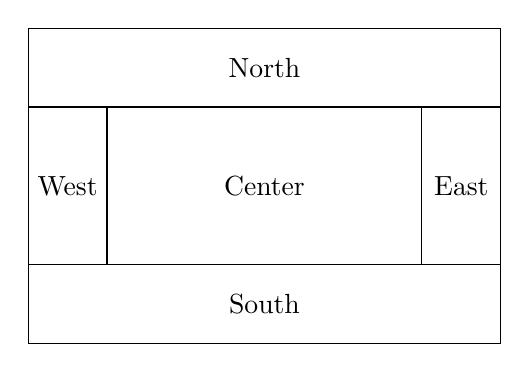
\begin{tikzpicture}[node distance=0cm, outer sep=0pt]
    \node (center) [rectangle, draw, minimum width=4cm, minimum height=2cm] {Center};
    \node (north) [rectangle, draw, minimum width=6cm, minimum height=1cm, above=of center, anchor=south] {North};
    \node (south) [rectangle, draw, minimum width=6cm, minimum height=1cm, below=of center, anchor=north] {South};
    \node (west) [rectangle, draw, minimum width=1cm, minimum height=2cm, left=of center, anchor=east] {West};
    \node (east) [rectangle, draw, minimum width=1cm, minimum height=2cm, right=of center, anchor=west] {East};
\end{tikzpicture}
\captionof{figure}{BorderLayout Regions}
\end{center}
\end{solutionbox}

\begin{mnemonicbox}
\mnemonic{FBGCBG Layouts = Flow Border Grid Card Box GridBag}
\end{mnemonicbox}

\questionmarks{2(a)}{3}{List out and explain steps to connect database.}

\begin{solutionbox}
\textbf{Database Connection Steps:}
\begin{center}
\begin{tabulary}{\linewidth}{|L|L|}
\hline
\textbf{Step} & \textbf{Action} \\ \hline
1. Load Driver & \code{Class.forName("driver.class")} \\ \hline
2. Create Connection & \code{DriverManager.getConnection()} \\ \hline
3. Create Statement & \code{connection.createStatement()} \\ \hline
4. Execute Query & \code{statement.executeQuery()} \\ \hline
5. Process Results & \code{resultSet.next()} \\ \hline
6. Close Resources & Close all connections \\ \hline
\end{tabulary}
\end{center}
\end{solutionbox}

\begin{mnemonicbox}
\mnemonic{LCD EPR = Load Create Driver, Execute Process Results}
\end{mnemonicbox}

\questionmarks{2(b)}{4}{Explain 3-tier architecture with diagram.}

\begin{solutionbox}
3-tier architecture separates application into three logical layers for better maintainability.

\begin{center}
\begin{tikzpicture}[node distance=2cm, auto]
    \node [gtu block] (UI) {Presentation Tier\\(Web Browser/UI)};
    \node [gtu block, right=of UI] (App) {Application Tier\\(Business Logic/Servlets)};
    \node [gtu block, right=of App] (Data) {Data Tier\\(Database Server)};
    
    \path [gtu arrow] (UI) -- (App);
    \path [gtu arrow] (App) -- (UI);
    \path [gtu arrow] (App) -- (Data);
    \path [gtu arrow] (Data) -- (App);
\end{tikzpicture}
\captionof{figure}{3-Tier Architecture}
\end{center}

\begin{center}
\begin{tabulary}{\linewidth}{|L|L|}
\hline
\textbf{Tier} & \textbf{Responsibility} \\ \hline
\textbf{Presentation} & User interface and user interaction \\ \hline
\textbf{Application} & Business logic and processing \\ \hline
\textbf{Data} & Data storage and management \\ \hline
\end{tabulary}
\end{center}

\begin{itemize}
    \item \textbf{Advantage}: Better scalability and maintainability.
    \item \textbf{Example}: Web browser $\rightarrow$ Web server $\rightarrow$ Database.
\end{itemize}
\end{solutionbox}

\begin{mnemonicbox}
\mnemonic{PAD = Presentation Application Data}
\end{mnemonicbox}

\questionmarks{2(c)}{7}{Describe JDBC API with interfaces and classes.}

\begin{solutionbox}
\textbf{JDBC API Components:}

\begin{center}
\captionof{table}{JDBC Components}
\begin{tabulary}{\linewidth}{|L|L|L|}
\hline
\textbf{Type} & \textbf{Component} & \textbf{Purpose} \\ \hline
Interface & Connection & Database connection \\ \hline
Interface & Statement & SQL execution \\ \hline
Interface & ResultSet & Query results \\ \hline
Interface & PreparedStatement & Precompiled SQL \\ \hline
Class & DriverManager & Driver management \\ \hline
Class & SQLException & Error handling \\ \hline
\end{tabulary}
\end{center}

\textbf{JDBC Architecture:}
\begin{center}
\begin{tikzpicture}[node distance=1.5cm, auto]
    \node [gtu block] (App) {Java Application};
    \node [gtu block, right=of App] (Api) {JDBC API};
    \node [gtu block, right=of Api] (Mgr) {JDBC Driver Manager};
    \node [gtu block, below=of Mgr] (Drv) {JDBC Driver};
    \node [gtu block, below=of Drv] (Db) {Database};
    
    \path [gtu arrow] (App) -- (Api);
    \path [gtu arrow] (Api) -- (Mgr);
    \path [gtu arrow] (Mgr) -- (Drv);
    \path [gtu arrow] (Drv) -- (Db);
\end{tikzpicture}
\captionof{figure}{JDBC Architecture}
\end{center}
\end{solutionbox}

\begin{mnemonicbox}
\mnemonic{CSRP Classes = Connection Statement ResultSet PreparedStatement}
\end{mnemonicbox}

\questionmarks{2(a OR)}{3}{List out advantages and disadvantages of JDBC.}

\begin{solutionbox}
\begin{center}
\captionof{table}{Advantages vs Disadvantages}
\begin{tabulary}{\linewidth}{|L|L|}
\hline
\textbf{Advantages} & \textbf{Disadvantages} \\ \hline
Platform Independent & Performance Overhead \\ \hline
Standard API & Complex Configuration \\ \hline
Multiple Database Support & Limited ORM Features \\ \hline
\end{tabulary}
\end{center}
\end{solutionbox}

\begin{mnemonicbox}
\mnemonic{PSM vs PCL = Platform Standard Multiple vs Performance Complex Limited}
\end{mnemonicbox}

\questionmarks{2(b OR)}{4}{Explain 2-tier architecture with diagram.}

\begin{solutionbox}
2-tier architecture directly connects client to database server.

\begin{center}
\begin{tikzpicture}[node distance=3cm, auto]
    \node [gtu block] (Client) {Client Tier\\(Application/UI)};
    \node [gtu block, right=of Client] (Data) {Data Tier\\(Database Server)};
    
    \path [gtu arrow] (Client) -- (Data);
    \path [gtu arrow] (Data) -- (Client);
\end{tikzpicture}
\captionof{figure}{2-Tier Architecture}
\end{center}

\begin{itemize}
    \item \textbf{Advantage}: Simple architecture, direct communication.
    \item \textbf{Disadvantage}: Limited scalability, tight coupling.
    \item \textbf{Example}: Desktop application connecting directly to database.
\end{itemize}
\end{solutionbox}

\begin{mnemonicbox}
\mnemonic{CD = Client Data (direct connection)}
\end{mnemonicbox}

\questionmarks{2(c OR)}{7}{List out JDBC driver types and Explain TYPE-4.}

\begin{solutionbox}
\textbf{JDBC Driver Types:}
\begin{center}
\captionof{table}{Driver Types}
\begin{tabulary}{\linewidth}{|L|L|L|}
\hline
\textbf{Type} & \textbf{Name} & \textbf{Description} \\ \hline
Type-1 & JDBC-ODBC Bridge & Uses ODBC driver \\ \hline
Type-2 & Native-API Driver & Part Java, part native \\ \hline
Type-3 & Network Protocol Driver & Pure Java, middleware \\ \hline
Type-4 & Native Protocol Driver & Pure Java, direct \\ \hline
\end{tabulary}
\end{center}

\textbf{TYPE-4 Driver Explanation:}
\begin{itemize}
    \item \textbf{Pure Java}: Completely written in Java.
    \item \textbf{Direct Communication}: Directly communicates with database.
    \item \textbf{Platform Independent}: No native libraries required.
    \item \textbf{Best Performance}: Fastest among all types.
    \item \textbf{Examples}: MySQL Connector/J, PostgreSQL JDBC.
\end{itemize}

\begin{center}
\begin{tikzpicture}[node distance=2cm, auto]
    \node [gtu block] (App) {Java Application};
    \node [gtu block, right=of App] (Driver) {Type-4 JDBC Driver\\(Pure Java)};
    \node [gtu block, right=of Driver] (Db) {Database Server};
    
    \path [gtu arrow] (App) -- (Driver);
    \path [gtu arrow] (Driver) -- (Db);
\end{tikzpicture}
\captionof{figure}{Type-4 Driver}
\end{center}
\end{solutionbox}

\begin{mnemonicbox}
\mnemonic{ONNN Drivers = ODBC Native Network Native-pure}
\end{mnemonicbox}

\questionmarks{3(a)}{3}{Explain Application of servlet.}

\begin{solutionbox}
\textbf{Servlet Applications:}
\begin{center}
\begin{tabulary}{\linewidth}{|L|L|}
\hline
\textbf{Application} & \textbf{Usage} \\ \hline
Web Forms & Process HTML form data \\ \hline
Database Operations & Connect and manipulate database \\ \hline
Session Management & Track user sessions \\ \hline
File Upload & Handle file uploads \\ \hline
\end{tabulary}
\end{center}
\end{solutionbox}

\begin{mnemonicbox}
\mnemonic{WDSF = Web Database Session File}
\end{mnemonicbox}

\questionmarks{3(b)}{4}{Explain difference between Applet and Servlet.}

\begin{solutionbox}
\begin{center}
\captionof{table}{Applet vs Servlet}
\begin{tabulary}{\linewidth}{|L|L|L|}
\hline
\textbf{Feature} & \textbf{Applet} & \textbf{Servlet} \\ \hline
\textbf{Execution} & Client-side (browser) & Server-side (web server) \\ \hline
\textbf{Purpose} & User interface & Request processing \\ \hline
\textbf{Security} & Restricted (sandbox) & Full server access \\ \hline
\textbf{Performance} & Limited by client & Server resources \\ \hline
\end{tabulary}
\end{center}
\end{solutionbox}

\begin{mnemonicbox}
\mnemonic{Client vs Server = Applet vs Servlet}
\end{mnemonicbox}

\questionmarks{3(c)}{7}{Explain life cycle of a servlet in detail.}

\begin{solutionbox}
\textbf{Servlet Life Cycle:}

\begin{center}
\begin{tikzpicture}[node distance=1.5cm, auto]
    \node [gtu state] (Load) {Load Class};
    \node [gtu state, right=of Load] (Init) {init()};
    \node [gtu state, below=of Init] (Serv) {service()};
    \node [gtu state, left=of Serv] (Dest) {destroy()};
    \node [gtu state, left=of Dest] (Unload) {Unload};
    
    \path [gtu arrow] (Load) -- (Init);
    \path [gtu arrow] (Init) -- (Serv);
    \path [gtu arrow] (Serv) edge [loop below] node {Requests} (Serv);
    \path [gtu arrow] (Serv) -- (Dest);
    \path [gtu arrow] (Dest) -- (Unload);
\end{tikzpicture}
\captionof{figure}{Servlet Life Cycle}
\end{center}

\begin{center}
\captionof{table}{Life Cycle Phases}
\begin{tabulary}{\linewidth}{|L|L|L|}
\hline
\textbf{Phase} & \textbf{Method} & \textbf{Description} \\ \hline
Loading & - & Web container loads servlet class \\ \hline
Initialization & \code{init()} & Called once, setup resources \\ \hline
Service & \code{service()} & Handles each request (doGet/doPost) \\ \hline
Destruction & \code{destroy()} & Cleanup before unloading \\ \hline
\end{tabulary}
\end{center}

\begin{itemize}
    \item \textbf{Thread Safety}: Multiple requests handled concurrently.
    \item \textbf{Single Instance}: One servlet instance handles all requests.
\end{itemize}
\end{solutionbox}

\begin{mnemonicbox}
\mnemonic{LISD = Load Init Service Destroy}
\end{mnemonicbox}

\questionmarks{3(a OR)}{3}{Explain web.xml file in servlet.}

\begin{solutionbox}
\textbf{web.xml Purpose:}
\begin{center}
\begin{tabulary}{\linewidth}{|L|L|}
\hline
\textbf{Element} & \textbf{Description} \\ \hline
Deployment Descriptor & Configuration file for web application \\ \hline
Servlet Mapping & Maps URL patterns to servlets \\ \hline
Initialization & Servlet parameters and load order \\ \hline
\end{tabulary}
\end{center}

\begin{itemize}
    \item \textbf{Location}: WEB-INF directory
    \item \textbf{Format}: XML configuration file
\end{itemize}
\end{solutionbox}

\begin{mnemonicbox}
\mnemonic{DMI = Deployment Mapping Initialization}
\end{mnemonicbox}

\questionmarks{3(b OR)}{4}{List out and Explain feature of servlet.}

\begin{solutionbox}
\textbf{Servlet Features:}
\begin{center}
\begin{tabulary}{\linewidth}{|L|L|}
\hline
\textbf{Feature} & \textbf{Description} \\ \hline
Platform Independent & Write once, run anywhere \\ \hline
Server-side & Executes on web server \\ \hline
Protocol Independent & Supports HTTP, FTP, etc. \\ \hline
Persistent & Stays in memory between requests \\ \hline
Secure & Built-in security features \\ \hline
\end{tabulary}
\end{center}
\end{solutionbox}

\begin{mnemonicbox}
\mnemonic{PSPPS = Platform Server Protocol Persistent Secure}
\end{mnemonicbox}

\questionmarks{3(c OR)}{7}{Explain session tracking in servlet.}

\begin{solutionbox}
\textbf{Session Tracking Methods:}
\begin{center}
\begin{tabulary}{\linewidth}{|L|L|}
\hline
\textbf{Method} & \textbf{Description} \\ \hline
Cookies & Small data stored in browser \\ \hline
URL Rewriting & Session ID in URL \\ \hline
Hidden Form Fields & Session data in forms \\ \hline
HttpSession & Server-side session object \\ \hline
\end{tabulary}
\end{center}

\textbf{HttpSession Logic Flow:}
\begin{center}
\begin{tikzpicture}[node distance=1.5cm, auto]
    \node [gtu state] (Start) {Request};
    \node [gtu state, right=of Start] (Check) {Check Session ID};
    \node [gtu decision, right=of Check] (Exists) {Exists?};
    \node [gtu state, below=of Exists] (New) {Create New};
    \node [gtu state, right=of Exists, node distance=3cm] (Use) {Use Existing};
    \node [gtu state, below=of Use] (Process) {Process};
    
    \path [gtu arrow] (Start) -- (Check);
    \path [gtu arrow] (Check) -- (Exists);
    \path [gtu arrow] (Exists) -- node {No} (New);
    \path [gtu arrow] (Exists) -- node {Yes} (Use);
    \path [gtu arrow] (New) -- (Process);
    \path [gtu arrow] (Use) -- (Process);
\end{tikzpicture}
\captionof{figure}{Session Tracking Logic}
\end{center}

\textbf{HttpSession Implementation:}
\begin{lstlisting}[language=Java]
HttpSession session = request.getSession();
session.setAttribute("user", username);
String user = (String) session.getAttribute("user");
\end{lstlisting}
\end{solutionbox}

\begin{mnemonicbox}
\mnemonic{CUHH = Cookies URL Hidden HttpSession}
\end{mnemonicbox}

\questionmarks{4(a)}{3}{Explain architecture of JSP with diagram.}

\begin{solutionbox}
\textbf{JSP Architecture:}
\begin{center}
\begin{tikzpicture}[node distance=1.5cm, auto]
    \node [gtu block] (JSP) {JSP Page};
    \node [gtu block, right=of JSP] (Engine) {JSP Engine};
    \node [gtu block, below=of Engine] (Servlet) {Servlet Gen};
    \node [gtu block, left=of Servlet] (Byte) {Compile};
    \node [gtu block, below=of Byte] (Exec) {Execute};
    \node [gtu block, right=of Exec] (Resp) {HTML Resp};
    
    \path [gtu arrow] (JSP) -- (Engine);
    \path [gtu arrow] (Engine) -- (Servlet);
    \path [gtu arrow] (Servlet) -- (Byte);
    \path [gtu arrow] (Byte) -- (Exec);
    \path [gtu arrow] (Exec) -- (Resp);
\end{tikzpicture}
\captionof{figure}{JSP Processing}
\end{center}

\begin{enumerate}
    \item \textbf{JSP Engine}: Translates JSP to servlet.
    \item \textbf{Web Container}: Manages JSP lifecycle.
    \item \textbf{Generated Servlet}: Actual execution unit.
\end{enumerate}
\end{solutionbox}

\begin{mnemonicbox}
\mnemonic{JSP = Java Server Pages (Page to Servlet)}
\end{mnemonicbox}

\questionmarks{4(b)}{4}{Explain JSP scripting elements with example.}

\begin{solutionbox}
\textbf{JSP Scripting Elements:}
\begin{center}
\captionof{table}{Scripting Elements}
\begin{tabulary}{\linewidth}{|L|L|L|}
\hline
\textbf{Element} & \textbf{Syntax} & \textbf{Purpose} \\ \hline
Scriptlet & \code{<\% code \%>} & Java code block \\ \hline
Expression & \code{<\%= expression \%>} & Output value \\ \hline
Declaration & \code{<\%! declaration \%>} & Variables/methods \\ \hline
\end{tabulary}
\end{center}

\textbf{Examples:}
\begin{lstlisting}[language=Java]
<%! int count = 0; %>               <!-- Declaration -->
<% count++; %>                      <!-- Scriptlet -->
<%= "Count: " + count %>            <!-- Expression -->
\end{lstlisting}
\end{solutionbox}

\begin{mnemonicbox}
\mnemonic{SED = Scriptlet Expression Declaration}
\end{mnemonicbox}

\questionmarks{4(c)}{7}{Explain JSP life cycle.}

\begin{solutionbox}
\textbf{JSP Life Cycle Phases:}

\begin{center}
\begin{tikzpicture}[node distance=1.5cm, auto]
    \node [gtu state] (Trans) {Translate};
    \node [gtu state, right=of Trans] (Comp) {Compile};
    \node [gtu state, right=of Comp] (Load) {Load};
    \node [gtu state, below=of Load] (Inst) {Instance};
    \node [gtu state, left=of Inst] (Init) {Init};
    \node [gtu state, left=of Init] (Serv) {Service};
    \node [gtu state, below=of Serv] (Dest) {Destroy};
    
    \path [gtu arrow] (Trans) -- (Comp);
    \path [gtu arrow] (Comp) -- (Load);
    \path [gtu arrow] (Load) -- (Inst);
    \path [gtu arrow] (Inst) -- (Init);
    \path [gtu arrow] (Init) -- (Serv);
    \path [gtu arrow] (Serv) edge [loop above] node {} (Serv);
    \path [gtu arrow] (Serv) -- (Dest);
\end{tikzpicture}
\captionof{figure}{JSP Life Cycle}
\end{center}

\begin{center}
\begin{tabulary}{\linewidth}{|L|L|}
\hline
\textbf{Phase} & \textbf{Description} \\ \hline
Translation & JSP converted to servlet source \\ \hline
Compilation & Servlet source compiled to bytecode \\ \hline
Loading & Servlet class loaded by JVM \\ \hline
Instantiation & Servlet object created \\ \hline
Initialization & \code{jspInit()} method called \\ \hline
Request Processing & \code{\_jspService()} handles requests \\ \hline
Destruction & \code{jspDestroy()} cleanup method \\ \hline
\end{tabulary}
\end{center}
\end{solutionbox}

\begin{mnemonicbox}
\mnemonic{TCLIIRD = Translation Compilation Loading Instantiation Init Request Destroy}
\end{mnemonicbox}

\questionmarks{4(a OR)}{3}{Explain difference between JSP and Servlet.}

\begin{solutionbox}
\begin{center}
\captionof{table}{JSP vs Servlet}
\begin{tabulary}{\linewidth}{|L|L|L|}
\hline
\textbf{Feature} & \textbf{JSP} & \textbf{Servlet} \\ \hline
\textbf{Code Style} & HTML with Java & Pure Java code \\ \hline
\textbf{Development} & Easier for UI & Better for logic \\ \hline
\textbf{Compilation} & Automatic & Manual \\ \hline
\textbf{Modification} & No recompilation needed & Requires recompilation \\ \hline
\end{tabulary}
\end{center}
\end{solutionbox}

\begin{mnemonicbox}
\mnemonic{HTML vs Java = JSP vs Servlet}
\end{mnemonicbox}

\questionmarks{4(b OR)}{4}{List out and Explain advantage of JSP.}

\begin{solutionbox}
\textbf{JSP Advantages:}
\begin{center}
\begin{tabulary}{\linewidth}{|L|L|}
\hline
\textbf{Advantage} & \textbf{Description} \\ \hline
Easy Development & HTML-like syntax with Java \\ \hline
Automatic Compilation & No manual compilation needed \\ \hline
Platform Independent & Runs on any Java-enabled server \\ \hline
Separation of Concerns & Design separated from logic \\ \hline
Reusable Components & Tag libraries and beans \\ \hline
\end{tabulary}
\end{center}
\end{solutionbox}

\begin{mnemonicbox}
\mnemonic{EAPSR = Easy Automatic Platform Separation Reusable}
\end{mnemonicbox}

\questionmarks{4(c OR)}{7}{What is cookie? Explain how to Read and delete cookie using JSP page.}

\begin{solutionbox}
\textbf{Cookie Overview:}
Cookie is a small piece of data stored on client's browser to maintain state.

\textbf{Cookie Operations:}
\begin{center}
\begin{tabulary}{\linewidth}{|L|L|}
\hline
\textbf{Operation} & \textbf{JSP Code} \\ \hline
Create & \code{Cookie cookie = new Cookie("name", "value");} \\ \hline
Add & \code{response.addCookie(cookie);} \\ \hline
Read & \code{Cookie[] cookies = request.getCookies();} \\ \hline
Delete & \code{cookie.setMaxAge(0);} \\ \hline
\end{tabulary}
\end{center}

\textbf{Reading Cookie Example:}
\begin{lstlisting}[language=Java]
<%
Cookie[] cookies = request.getCookies();
if (cookies != null) {
    for (Cookie cookie : cookies) {
        if ("username".equals(cookie.getName())) {
            out.println("User: " + cookie.getValue());
        }
    }
}
%>
\end{lstlisting}

\textbf{Deleting Cookie Example:}
\begin{lstlisting}[language=Java]
<%
Cookie cookie = new Cookie("username", "");
cookie.setMaxAge(0);
response.addCookie(cookie);
%>
\end{lstlisting}
\end{solutionbox}

\begin{mnemonicbox}
\mnemonic{CARD = Create Add Read Delete}
\end{mnemonicbox}

\questionmarks{5(a)}{3}{Explain importance of MVC architecture.}

\begin{solutionbox}
\textbf{MVC Importance:}
\begin{center}
\begin{tabulary}{\linewidth}{|L|L|}
\hline
\textbf{Benefit} & \textbf{Description} \\ \hline
Separation of Concerns & Logic, presentation, data separated \\ \hline
Maintainability & Easy to modify individual components \\ \hline
Testability & Components can be tested independently \\ \hline
\end{tabulary}
\end{center}

\begin{itemize}
    \item \textbf{Code Organization}: Better structure and organization.
    \item \textbf{Team Development}: Multiple developers can work simultaneously.
\end{itemize}
\end{solutionbox}

\begin{mnemonicbox}
\mnemonic{SMT = Separation Maintainability Testability}
\end{mnemonicbox}

\questionmarks{5(b)}{4}{Explain Aspect oriented programming and dependency injection in brief.}

\begin{solutionbox}
\textbf{Aspect Oriented Programming (AOP):}
\begin{center}
\begin{tabulary}{\linewidth}{|L|L|}
\hline
\textbf{Concept} & \textbf{Description} \\ \hline
Cross-cutting Concerns & Logging, security, transactions \\ \hline
Aspects & Modular units of cross-cutting functionality \\ \hline
Join Points & Points where aspects are applied \\ \hline
\end{tabulary}
\end{center}

\textbf{Dependency Injection (DI):}
\begin{center}
\begin{tabulary}{\linewidth}{|L|L|}
\hline
\textbf{Concept} & \textbf{Description} \\ \hline
Inversion of Control & Dependencies provided externally \\ \hline
Loose Coupling & Objects don't create dependencies \\ \hline
Configuration & Dependencies configured externally \\ \hline
\end{tabulary}
\end{center}
\end{solutionbox}

\begin{mnemonicbox}
\mnemonic{AOP = Aspects Over Points, DI = Dependencies Injected}
\end{mnemonicbox}

\questionmarks{5(c)}{7}{Explain MVC architecture.}

\begin{solutionbox}
\textbf{MVC Components:}

\begin{center}
\begin{tikzpicture}[node distance=2.5cm, auto]
    \node [gtu block] (View) {View\\(Presentation)};
    \node [gtu block, right=of View] (Ctrl) {Controller\\(LogicFlow)};
    \node [gtu block, right=of Ctrl] (Model) {Model\\(Data/Logic)};
    
    \path [gtu arrow] (View) edge[bend left] node {} (Ctrl);
    \path [gtu arrow] (Ctrl) edge[bend left] node {} (View);
    
    \path [gtu arrow] (Ctrl) edge[bend left] node {} (Model);
    \path [gtu arrow] (Model) edge[bend left] node {} (Ctrl);
\end{tikzpicture}
\captionof{figure}{MVC Interaction}
\end{center}

\begin{center}
\begin{tabulary}{\linewidth}{|L|L|}
\hline
\textbf{Component} & \textbf{Responsibility} \\ \hline
Model & Business logic and data management \\ \hline
View & User interface and presentation \\ \hline
Controller & Request handling and flow control \\ \hline
\end{tabulary}
\end{center}

\textbf{MVC Flow:}
\begin{enumerate}
    \item \textbf{User Request} $\rightarrow$ Controller receives request.
    \item \textbf{Controller} $\rightarrow$ Processes request, calls Model.
    \item \textbf{Model} $\rightarrow$ Performs business logic, returns data.
    \item \textbf{Controller} $\rightarrow$ Selects appropriate View.
    \item \textbf{View} $\rightarrow$ Renders response to user.
\end{enumerate}
\end{solutionbox}

\begin{mnemonicbox}
\mnemonic{MVC = Model View Controller (Business UI Control)}
\end{mnemonicbox}

\questionmarks{5(a OR)}{3}{Explain advantages of MVC architecture.}

\begin{solutionbox}
\textbf{MVC Advantages:}
\begin{center}
\begin{tabulary}{\linewidth}{|L|L|}
\hline
\textbf{Advantage} & \textbf{Description} \\ \hline
Code Reusability & Components can be reused across applications \\ \hline
Parallel Development & Multiple developers work on different layers \\ \hline
Easy Testing & Each component tested independently \\ \hline
Maintenance & Changes in one layer don't affect others \\ \hline
\end{tabulary}
\end{center}
\end{solutionbox}

\begin{mnemonicbox}
\mnemonic{CPEM = Code Parallel Easy Maintenance}
\end{mnemonicbox}

\questionmarks{5(b OR)}{4}{Explain difference between spring and spring boot.}

\begin{solutionbox}
\begin{center}
\captionof{table}{Spring vs Spring Boot}
\begin{tabulary}{\linewidth}{|L|L|L|}
\hline
\textbf{Feature} & \textbf{Spring} & \textbf{Spring Boot} \\ \hline
Configuration & Manual XML/Java config & Auto-configuration \\ \hline
Setup Time & More setup required & Minimal setup \\ \hline
Embedded Server & External server needed & Built-in server \\ \hline
Dependencies & Manual dependency management & Starter dependencies \\ \hline
\end{tabulary}
\end{center}
\end{solutionbox}

\begin{mnemonicbox}
\mnemonic{Manual vs Auto = Spring vs SpringBoot}
\end{mnemonicbox}

\questionmarks{5(c OR)}{7}{Explain architecture of Spring framework.}

\begin{solutionbox}
\textbf{Spring Framework Architecture:}

\begin{center}
\begin{tikzpicture}[node distance=2cm, auto]
    \node [gtu block] (Core) {Core Container\\(IoC \& DI)};
    \node [gtu block, right=of Core] (Web) {Web Layer\\(MVC, WebFlux)};
    \node [gtu block, below=of Core] (Data) {Data Access\\(JDBC, ORM)};
    \node [gtu block, right=of Data] (Test) {Test\\(JUnit, Mock)};
    \node [gtu block, below=of Data] (AOP) {AOP\\(Aspects)};
    
    \path [gtu arrow] (Core) -- (Web);
    \path [gtu arrow] (Core) -- (Data);
    \path [gtu arrow] (Core) -- (AOP);
    \path [gtu arrow] (Core) -- (Test);
\end{tikzpicture}
\captionof{figure}{Spring Architecture}
\end{center}

\textbf{Spring Modules:}
\begin{center}
\begin{tabulary}{\linewidth}{|L|L|}
\hline
\textbf{Module} & \textbf{Purpose} \\ \hline
Core Container & IoC container, dependency injection \\ \hline
Data Access & JDBC, ORM, transaction management \\ \hline
Web & Web MVC, REST services \\ \hline
AOP & Aspect-oriented programming \\ \hline
Test & Testing support and mock objects \\ \hline
\end{tabulary}
\end{center}
\end{solutionbox}

\begin{mnemonicbox}
\mnemonic{CDWAST = Core Data Web AOP Security Test}
\end{mnemonicbox}

\end{document}
